\chapter{Background}
% Studenten visar kännedom om teoretisk bakgrund och tidigare utfört arbete (betydande litteratur nämns och relevant material används).
% Bakgrunden är sammanhängande och relevant.
This Chapter will present some background knowledge with needed information to comprehend the chapters to follow. The chapter starts with a general description about \textit{Web Application} structure and is followed by a section with the two most common \textit{Security Vulnerabilities} to a web application. After those sections follows  two sections describing \textit{Dynamic Taint Propagation} and \textit{Domain Driven Security}. The last section is a chapter about \textit{Java Instrumentation}.


\section{Web Application}
To make applications available for a large set off people and also make the application accessible from, now days, almost everywhere do businesses deploy their applications to the web. They deployment of an application can vary a lot but the most common architectural structure for a web application is based on a three tier architecture. The first is the presentation tire which is the visual components rendered by a browser. The second is the logic tire which can be seen as the brain of the application. The last and third is the storage tier, where the second tier can store data as needed. \parencite{JustinClarke-Salt2009SIAa} An illustration of the three layer architecture can be seen in figure \ref{fig:webApplication-Haldar}.

\begin{figure}
  \centering
  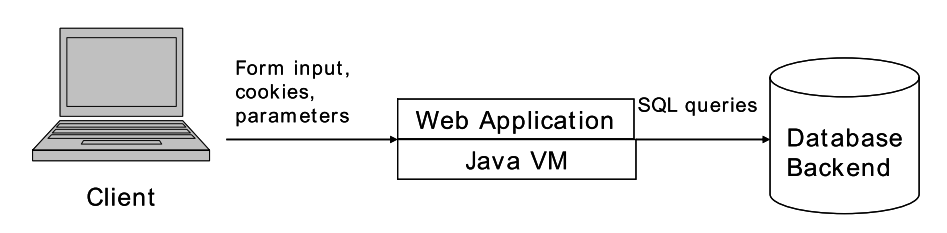
\includegraphics[width=\textwidth]{images/webApplication-Haldar.png}
  \caption{Web application structure \cite{Haldar}.}
  \label{fig:webApplication-Haldar}
\end{figure}

As can be seen in figure \ref{fig:webApplication-Haldar} dose the tiers only communicate with the tire closest to itself. This causes the second tier to become a safe guard for tier three where the valuable and possibly sensitive information is stored. The storage tier contains all the information the application needs to provide the wanted service. Such information might for example be name, email, personal number and credit card information. \parencite{JustinClarke-Salt2009SIAa}


\subsection{Structured Query Language}
The communication between tier two and tier three is done trough a standardize language called Structured Query Language, mostly known as SQL. SQL is created to programmatically manipulate and access databases. The vast majority of todays database uses SQL. The language works by building queries specifying the wanted information or task. The query will be evaluated and handled up upon by the SQL engine. \parencite{DarieCristian2003TPGt}


\section{Security Vulnerabilities}
The organization Open Web Applications Security Project, mostly known for its shortening (OWASP), is a online community which aim to provide knowledge how to to secure web applications. \parencite{OpenWebApplicationSecurityProject} OWASP have produced reports about the top 10 security risks with a web application and the latest was published 2017. The report contains information about the ten most common application security risks that for the current year. Information such as how the security risk is exploited and possible prevention method is also presented. This thesis will look at security risk number one and eight which is Injection Attacks and Cross-site Scripting. \parencite{OWASP2017}


\subsection{Injection}
The most common security risk is Injection Attacks. \parencite{OWASP2017} A Injection Attack is any attack where the attacker's input changes the intent of the execution. Common result of Injection Attacks are file destruction, lack of accountability, denial of access and data loss. \parencite{Secure_Web}

Injection Attacks can be divided into two different subgroups. These two subgroups are SQL Injection and Blind SQL Injection. \parencite{Secure_Web}


\subsubsection{SQL Injection}
SQL Injection is when a SQL query is tampered which results in gaining content from the database which was not intended. Listing \ref{lst:acceptable_to_SQL_Injection} displays a SQL Query which is open to SQL Injections. This is due to the fact that the variable UserId is never validated before it is propagated into the query. \parencite{JustinClarke-Salt2009SIAa, Secure_Web} 

\hfill
\begin{lstlisting}[
  language=SQL,
  caption=Code Acceptable to SQL Injection,
  label={lst:acceptable_to_SQL_Injection}]
userId = (*@\textit{userInput}@*)
"SELECT * FROM Users WHERE userId = " + userId
\end{lstlisting}
\hfill

The query will work as intended as long as the user input, notated with \textit{userInput}, only is a valid Integer (since Integer is what we have decided that user id is in this application). But what happens if the user input is \textit{10 or 1 = 1}? This user input would result in the query seen in listing \ref{lst:SQL_Injection}.

\hfill
\begin{lstlisting}[
  language=SQL,
  caption=SQL Injection,
  label={lst:SQL_Injection}]
SELECT * FROM Users WHERE userId = 10 or 1 = 1
\end{lstlisting}
\hfill

This query would result in query that always evaluates to true. The result of this will be that the query returns the whole table of users. This problem can be prevented in a couple of different ways. The first is through validation of the input. By verifying the input as seen in listing \ref{lst:SQL_Injection_Verified} can we protect the query from being assessable to SQL Injection.

\hfill
\begin{lstlisting}[
  language=SQL,
  caption=Preventing SQL Injection through Verification,
  label={lst:SQL_Injection_Verified}]
userId = (*@\textit{userInput}@*)
isInteger(userId)
"SELECT * FROM Users WHERE userId = " + userId
\end{lstlisting}
\hfill

A second more common alternative is to use SQL Parameters which handles the verification for the user. This leaves the verification and validation of input up to the SQL engine. A example written with SQL Parameters can be seen in listing \ref{lst:SQL_Injection_Parameters}.

\hfill
\begin{lstlisting}[
  language=SQL,
  caption=Preventing SQL Injection through SQL Parameters,
  label={lst:SQL_Injection_Parameters}]
userId = (*@\textit{userInput}@*)
sqlQuery = "SELECT * FROM Users WHERE userId = @0"
db.Execute(sqlQuery, userId)
\end{lstlisting}


\subsubsection{Blind SQL Injection}
Blind SQL Injection is very similar to SQL Injection. The only difference is that that attacker dose not receive the wanted information from the database. The information is instead received by monitoring variables such as how long time the response took or what kind of error messages it returns. A example of the first is a SQL query that tells the SQL engine to sleep depending on a condition. A example of this can be seen in listing \ref{lst:Blind_SQL_Injection_Time}. \parencite{JustinClarke-Salt2009SIAa, Secure_Web} 

\hfill
\begin{lstlisting}[
  language=SQL,
  caption=Time Based Blind SQL Injection,
  label={lst:Blind_SQL_Injection_Time},
  xleftmargin=-0.8cm]
SELECT * FROM Users WHERE userId = 1 WAITFOR DELAY '0:0:5'
\end{lstlisting}
\hfill

The second variant of Blind SQL Injection, which is by analyzing the error messages, and depending on what they return build a image off the wanted answer. This is mostly done by testing different combination of true and false questions. \parencite{JustinClarke-Salt2009SIAa, Secure_Web} 


\subsection{Cross-site Scripting}
Cross-Site Scripting (XSS) have been a vulnerability since the beginning of the internet. One of the first XSS attacks was created just after the release of JavaScript. The attack was conducted trough loading a malicious web application into a frame on the site that the attacker want to gain information of. The attacker could then through JavaScript access any content that is visible or typed into the web application. To prevent this form of attack were the standard of Same-Origin Policy introduced. Same-Origin Policy restricts JavaScript to only access content from its own origin. \parencite{FogieSeth2007Xacs, w3csop}

But the introduction of the Same-Origin Policy did not stop the attackers from preforming XSS attacks. The next wave of attacks were mostly towards chat rooms where it was possible to inject malicious scripts into the input of the message. Which would then later be reflected by the server itself, when displaying the message for other users, and thereby bypassing the Same-Origin Policy. \parencite{FogieSeth2007Xacs}

XSS can be divided into three different sub categories. Which are: reflected, Stored and DOM Based XSS.

\subsubsection{Reflected XSS}
Reflected XSS is mostly conducted trough a malicious link that an unknowing user clicks. The malicious link will exploit a vulnerable input on the targeted web application and though the input reflect back content to the user. \parencite{Secure_Web}


\subsubsection{Stored XSS}
Stored XSS is when malicious scripts is stored in the targeted web applications database. This malicious script is then loaded and presented for each user which is trying to access the application. \parencite{Secure_Web}


\subsubsection{DOM Based XSS}
DOM Based XSS is very similar to Reflected XSS but it dose not necessary have to be reflected from the application server. DOM Based XSS modifies the DOM tree and is able to exploit the user. \parencite{Secure_Web}


\section{Dynamic Taint Propagation}
Taint Propagation, also known as taint analysis and taint checking, is a tool to analyse the flow of information in a domain. \parencite{Pan2015} It works by giving input data a tainted property which follows the data and propagates onto other data which it comes in contact with. Tainted data can be detainted. This is done by validating the data. The taint property is later checked in security sensitive sinks. \parencite{Pan2015} Taint Propagation can be done in two different ways: Static and dynamic. The static is a evaluation tool which is done statically and before runtime. Dynamic Taint Propagation is a tool that is executing in runtime. Dynamic Taint Propagation works by actively blocking any data that is trying to enter the sink. This thesis will not be handle the Static version of Taint Propagation. 

Perl and Ruby are two programming languages which have adapted to user Dynamic Taint Checking. \parencite{perl, ruby} And there are some tools who enables taint checking for other languages such as TaintDroid \parencite{Ma2010} and FlexTaint \parencite{Venkataramani2008}.

As named earlier is two of OWASP's top 10 application security risks of 2017 Injection Attack and Cross-Site Scripting (XSS). \parencite{OWASP2017} Protection against these two attacks are best done by validating input data which Dynamic Taint Propagation helps to enforce.


\section{Domain Driven Security}
There exists a plethora of tools who aim to help in the process of developing complex domain models, but Domain Driven Design (DDD) is not one if them. \parencite{Bankes, 10.1007/978-3-319-24309-2_33} DDD is more of a thought process and methodology to follow every step of the process. \parencite{EvansEric2004Dd:t} In \emph{Domain-driven design reference: definitions and patterns summaries} do \textcite{evans_2015} describe DDD through three core ideas:

\begin{itemize}
  \item Focus on the core domain.
  \item Explore models in a creative collaboration of domain practitioners and software practitioners.
  \item Speak a ubiquitous language within an explicitly bounded context.
\end{itemize}

The core domain is the part of your product that is most important and often is your main selling point compared to other similar products. \parencite{millett_2015} A discussion and even possible a documentation describing the core domain is something that will help the development of the product. The idea is to keep everybody on the same track heading in the same direction. \parencite{EvansEric2004Dd:t}

The second idea is to explore and develop every model in collaboration between domain practitioners, who are experts in the given domain, and software developers. This ensures that important knowledge needed to successfully develope the product is communicated back and forth between the two parties. \parencite{millett_2015} The third idea is important to enable and streamline the second. By using a ubiquitous language will miscommunication between domain and software practitioners be minimized and the collaboration between the two parties can instead focus on the important parts which is to develop the product. \parencite{evans_2015}

\textcite{evans_2015} do as well argue about the weight of clearly defining the bounded contexts for each defined model, and this needs to be done in the ubiquitous language created for the specific product. The need of this exists because of the otherwise great risk of misunderstandings and erroneous assumptions in the collaborations between the different models. \parencite{millett_2015}

\textcite{Wilander2009, Johnsson2009} created 2009 a blog post each in a synchronous manner where they together introduces the concept of Domain Driven Security (DDS) to the public. They describe DDS as the intersection between DDD and application security. DDD is about developing complex domain models and one of the most basic rule of application security is to always validate input data. DDS in other hand, is about the importance of creating and maintaining domain models who are reflecting the product correctly and that they are validated so they cant be populated with erroneous data. \parencite{Wilander2009, Johnsson2009, Arnor2016, Stendahl2016}


\section{Java Instrumentation}
Java Instrumentation is a way to modify the execution of a application on the Java Virtual Machine (JVM) without having knowledge nor the need of modifying the application code itself. This makes it beneficial to implement for example monitoring agents and event loggers. Java Instrumentation works by modifying the bytecode of the JVM. \parencite{Java_Instrument} There exists a number of libraries that can help the developer in the task of instrumenting the JVM. The one that will be used in this thesis is called Javassist. Javassist provides a library that simplifies the task of editing and creating java class file at runtime. \parencite{Javassist}